\documentclass[11pt,a4paper]{article}
\usepackage[margin=25mm]{geometry}
\usepackage[T1]{fontenc}
\usepackage[utf8]{inputenc}
\usepackage[british]{babel}
\usepackage{lmodern,microtype,amsmath,amssymb,booktabs,tabularx,graphicx}
\usepackage{xcolor,listings,caption,placeins}
\usepackage[colorlinks=true,linkcolor=teal,citecolor=teal,urlcolor=teal]{hyperref}
\hypersetup{pdftitle={Solution to the challenge proposed by Doppel},
  pdfauthor={Alberto Hernandez-Espinosa},
  pdfsubject={An information-theoretic answer and an exact Boolean-network study}}
\definecolor{codebg}{HTML}{F3F6F8}
\lstset{language=Python,basicstyle=\ttfamily\footnotesize,backgroundcolor=\color{codebg},
  frame=none,breaklines=true,showstringspaces=false,columns=fullflexible,
  keepspaces=true,keywordstyle=\color{teal},commentstyle=\color{gray}}
\captionsetup{font=small,labelfont=bf}
\setlength{\parskip}{4pt}
\setlength{\parindent}{0pt}
\setlength{\emergencystretch}{2em}
\graphicspath{{generated/}}
\newcommand{\KL}{D_{\mathrm{KL}}}
\newcommand{\E}{\mathbb{E}}
\newcommand{\bits}{\{0,1\}}
\newcommand{\CDL}{L_{\mathrm{causal}}}
\title{Solution to the challenge proposed by Doppel\\[5pt]
  \large An information-theoretic answer and an exact Boolean-network study}
\author{Alberto Hernandez-Espinosa}
\date{13 September 2026}

\begin{document}
\maketitle

\begin{abstract}
Doppel's phishing challenge reached by means \textbf{3Blue1Brown}, asks which phrase frequencies maximise expected
payoff while remaining within a divergence-based alarm budget. The optimum
is an exponential reweighting of normal traffic, with its strength set by
the budget. I give the proof and boundary cases, then examine a constrained
version in which a Boolean network generates the distribution and the
attacker may change one connection. A ten-node example shows how the best
admissible payoff compares with the unrestricted bound. A verified study of
106,789 networks supports the computational construction. In the spirit
of Kolmogorov's algorithmic complexity, I use the length of an exact
generative programme as a secondary description of the mechanism.
\end{abstract}

\section{Introduction}
The challenge asks for an optimal distribution, given normal phrase
frequencies, phrase payoffs and a KL-divergence alarm rule~\cite{challenge}.
I solve this distributional problem analytically, including its boundary
cases. A Boolean-network experiment then evaluates the choices attainable
through specified structural changes, with exact enumeration at the
studied sizes. Programme length provides a secondary description of the
generating rules. These contributions distinguish the optimal frequency
mixture, the choices available to a constrained mechanism and the size of
its encoded representation. Supplementary material provides the full
implementation and experimental evidence.

\section{The challenge and its solution}
A phrase is a particular wording; a phrase category groups wordings
with a shared function. For example, \emph{reply quickly} and \emph{respond
today} could both express urgency. A message may contain phrases from
several categories, such as an offering together with urgency.
The original puzzle assigns probabilities to individual phrases.
Our Boolean-network extension instead represents a message by the
presence or absence of category features. Using the order offering,
request, urgency, $101$ denotes an offering and urgency without a request,
regardless of the particular wordings used.

I treat each complete combination as one message type. Its probability
describes those features occurring together: the distribution over types
is a joint distribution. One output is one combination, not a distribution
by itself. This extends the alphabet of the original puzzle while retaining
its mathematical form. Below, outcome $i$ denotes a phrase in the puzzle
or a complete combination in the extension. Let $q_i$ be its normal
frequency, $p_i$ its chosen frequency and $s_i\in[0,1]$ its specified success
probability when unflagged. A campaign is the collection of messages
evaluated together: $p_i=0.2$ means that outcome $i$ is selected in 20\%
of its messages on average. Probabilities of individual features need
not sum to one, since features can coexist; probabilities of the complete
types do. The payoff belongs to the complete outcome, not to a sum of
the phrases it contains.
Multiplying $p_i$ by $s_i$ weights that outcome's success by how often
it is used. Adding these contributions gives expected payoff per message.
The detector flags a campaign when $\KL(p\Vert q)>C$, where $C\geq0$
is the alarm budget. Treating a flagged campaign as receiving zero payoff,
the nonnegative payoffs and feasible baseline give the problem
\begin{equation}\label{eq:challenge}
 \max_p \sum_i p_i s_i
 \quad\text{subject to}\quad p_i\geq0,\quad \sum_i p_i=1,\quad
 \KL(p\Vert q)=\sum_i p_i\log\frac{p_i}{q_i}\leq C.
\end{equation}
The maximum asks for the best frequency mixture. Nonnegative entries
summing to one make it a probability distribution. In KL divergence,
$p_i/q_i$ compares a chosen frequency with normal traffic; the logarithm
of this ratio is averaged using $p$. The result is zero at $p=q$ and
positive otherwise. Thus the alarm limits a shift in frequencies, rather
than the success rate itself. Natural logarithms express $C$ in nats.
If $q_i=0$, using that outcome with positive probability gives infinite
KL. For finite $C$ we therefore set $p_i=0$ and restrict sums to $q_i>0$.
Terms with $p_i=0$ contribute zero. The puzzle uses exact distributions;
estimating them from a finite batch is a separate observation problem.

\subsection{The answer}
Reweight each baseline frequency by an exponential factor:
\begin{equation}\label{eq:tilt}
 p_i(\beta)=\frac{q_i e^{\beta s_i}}{Z(\beta)},
 \qquad Z(\beta)=\sum_j q_j e^{\beta s_j}.
\end{equation}
First multiply each normal frequency by $e^{\beta s_i}$, the exponential
of $\beta s_i$. A larger payoff receives a larger multiplier. Then add
all these weights to obtain $Z(\beta)$ and divide each weight by that
total. This normalisation makes the new frequencies sum to one.
The parameter $\beta$ controls how strongly payoffs affect the mixture:
at zero all multipliers are one and $p=q$. In the interior case,
increase $\beta$ until $\KL(p(\beta)\Vert q)=C$, using the available
alarm budget. The boundary cases below specify when this applies.

For an illustrative example, let $q=(0.5,0.3,0.2)$,
$s=(0.1,0.4,0.9)$ and $C=0.25$.
Then $\beta\approx2.09644$ and
$p\approx(0.23444,0.26383,0.50173)$. In 1,000 selections, the expected
outcome counts change from $(500,300,200)$ to approximately
$(234,264,502)$. The highest-payoff outcome becomes more frequent,
while the mixture remains at the alarm limit. Expected payoff rises
from $0.35$ to $0.580533$, calculated by multiplying each new frequency
by its payoff and adding. Appendix~\ref{app:interpretation} gives
further detail.

\subsection{Why it is optimal}
Write $\E_p[s]=\sum_i p_i s_i$ for expected payoff under $p$. To prove
optimality, compare any feasible mixture with $p(\beta)$. KL divergence
between them cannot be negative, so for $\beta>0$,
\begin{align}
 0\leq\KL(p\Vert p(\beta))
 &=\KL(p\Vert q)-\beta\E_p[s]+\log Z(\beta),\\
 \E_p[s]&\leq\frac{C+\log Z(\beta)}{\beta}.
\end{align}
The first line rewrites that nonnegative difference in terms of payoff
and divergence from normal traffic. Replacing the latter by its allowed
maximum $C$ gives the second line: a ceiling on every feasible payoff.
When $p=p(\beta)$ and its divergence equals $C$, both inequalities become
equalities. The proposed mixture reaches the ceiling and is optimal.
To find its weight, observe that
\begin{equation}
 \frac{d}{d\beta}\KL(p(\beta)\Vert q)
 =\beta\,\operatorname{Var}_{p(\beta)}(s).
\end{equation}
The derivative describes how divergence changes as $\beta$ increases.
The variance measures the spread of payoffs under the current mixture.
If the supported payoffs differ, this spread is positive for finite
$\beta$, so divergence increases strictly for $\beta>0$. We can therefore
find the unique interior weight by adjusting one number until the
divergence reaches $C$.

\subsection{Boundary cases}
At $C=0$, the only feasible distribution is $q$. If all supported payoffs
are equal, every feasible distribution is optimal. Otherwise, let $S_*$
contain the supported outcomes with largest payoff and let
$Q_*=\sum_{i\in S_*}q_i$, their combined frequency in normal traffic.
Within this set, $q_{S_*}(i)=q_i/Q_*$ preserves their relative normal
frequencies and rescales them to sum to one. For a mixture using only
these best outcomes,
\[
 \KL(p\Vert q)=\KL(p\Vert q_{S_*})-\log Q_*\geq-\log Q_*.
\]
The remaining KL term cannot be negative. Preserving those relative
frequencies makes it zero, so $-\log Q_*$ is the smallest budget
permitting maximum payoff.
For $C\geq-\log Q_*$, choose $p_i=q_i/Q_*$ on $S_*$ and zero elsewhere.
For $0<C<-\log Q_*$, the finite positive $\beta$ above attains the optimum.
A deterministic choice of a maximum-payoff outcome $k$ is also optimal
when $C\geq-\log q_k$: this is the divergence of using that outcome
every time. For the example above, using only outcome 3 requires
$-\log(0.2)\approx1.609$ nats, exceeding the budget of $0.25$.
Mixing is required in the interior case, but need not be required at
larger budgets.

\section{When a mechanism restricts the choice}
The unrestricted solution permits any feasible probability vector.
To examine a structural restriction, let a Boolean network update its
$N$ binary nodes synchronously by $x_{t+1}=F_A(x_t)$. Here $x_t$ is
the current vector of zeros and ones; $F_A$ applies the local gates
using connections recorded in $A$ to produce the next vector.
The one-step repertoire lists every possible input vector and its output.
An input is a generator state, rather than text submitted to a detector.
A permitted attack adds or removes one connection while keeping gate
types and parameters fixed. It changes an internal dependency and can
therefore change which states occur and how frequently.

Each node now represents one category feature and each complete output
one message type, as defined in Section~2. The gates model logical
dependencies in how combinations are generated. An AND rule, for example,
activates an output feature only when all its connected input features
are present; XOR activates it when an odd number are present. Shared
inputs and such rules can make output features dependent. This gives an
abstract model of rule-based composition, rather than independently
choosing every feature. The experimental rules and payoffs are declared
mathematical choices, without calibration to text or recipient responses.
The results therefore concern the generation and frequencies of abstract
message types; they do not establish grammatical validity, intelligence
or persuasive effectiveness.

Feeding each output back as the next input produces a trajectory.
There are only $2^N$ states; once a state repeats, the deterministic rules
repeat the same sequence, forming a cycle. Its basin contains every
initial state that eventually reaches it. To define the observed
distribution, start uniformly over all $2^N$ states and sample a phase
uniformly from the eventual cycle. If state $x$ lies on a cycle of length
$\ell$ whose basin contains $b$ initial states, then
\[
 \mu_A(x)=\frac{b}{2^N\ell}.
\]
The fraction $b/2^N$ is the chance of reaching that cycle under uniform
initialisation. Dividing by $\ell$ shares its probability equally among
its phases. Transient states receive zero long-run mass because their
finite visits contribute a vanishing fraction of an indefinitely long
trajectory; this does not imply rejection or failure. The detector uses
the resulting frequencies of whole combinations, rather than sequence
order. Counting outputs after one update with uniformly sampled inputs
gives a different observation: how many starting states produce each
combination immediately. Both distributions are joint across features;
cycles determine which combinations recur and their long-run weights.
Our distribution averages over initial states and cycle phases; one run
eventually visits only its own cycle. Appendix~\ref{app:dynamics} gives
the full observation convention.

The baseline network $A_0$ generates $q=\mu_{A_0}$ and each permitted
network $A$ generates $p=\mu_A$. The symbol $\mu$ denotes the frequencies
calculated from that network's cycles and basins; $q$ remains fixed
throughout the comparison. For a finite catalogue $\mathcal A$ of
nonidentity changes---actual modifications, excluding the unchanged
network---select
\[
 \max_{A\in\mathcal A:\,\KL(\mu_A\Vert\mu_{A_0})\leq C}
       \sum_x\mu_A(x)s(x).
\]
For every candidate, compute its distribution, discard it if its KL
exceeds $C$, and average its state payoffs $s(x)$ using the remaining
frequencies $\mu_A(x)$. The maximum selects the highest such average.
This is the original objective evaluated on a restricted set of choices.
If none is feasible, report the result as unavailable; taking no action
is excluded from this catalogue and can be added explicitly if desired.
Its optimum cannot exceed the unrestricted optimum because every
admissible network distribution is also a candidate in the unrestricted
problem.

\subsection{A ten-node example}
Figure~\ref{fig:network} shows the saved baseline
\texttt{ring\_n10\_s1000}. Its 1,024 initial states lead to one fixed point
and three eight-state cycles, with basin sizes 6, 148, 389 and 481.
For example, each state of the second cycle receives mass
$148/(1024\cdot8)=37/2048$; the fixed point 0 receives $6/1024$.
We obtain these counts by following the transitions from every initial
state and grouping those that reach the same cycle. The 148 starting
states give their cycle probability $148/1024$; its eight combinations
share that weight equally. There are 432 distinct one-step outputs but
only 25 states with positive long-run mass. Thus selecting the observation
scheme changes which message types receive probability. A structural
change can alter both cycle membership and basin sizes, changing those
probabilities even when some recurring combinations are retained.
The cycles, selected transitions and exact probability table appear in
Appendix~\ref{app:study}.

\begin{figure}[htbp]\centering
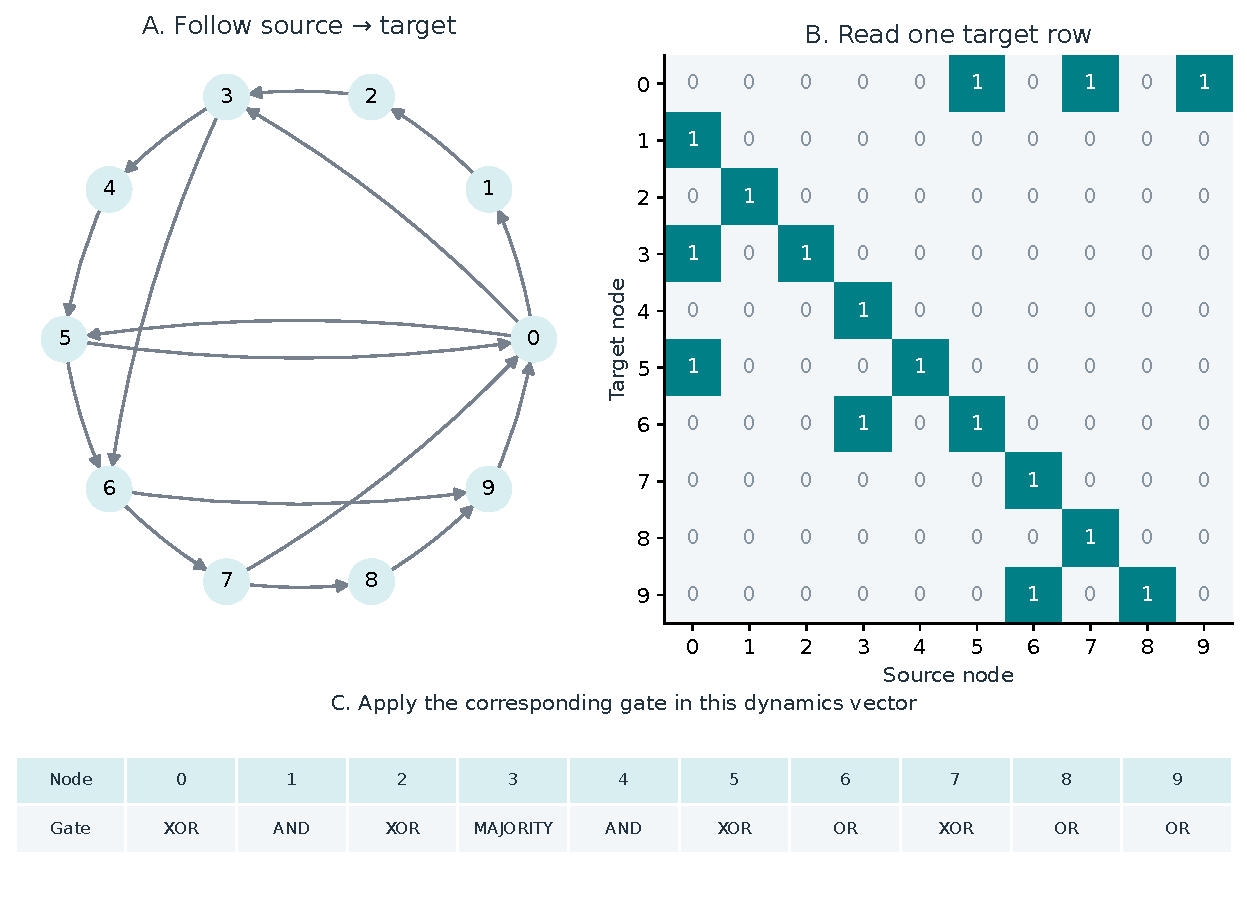
\includegraphics[width=.9\linewidth]{network.pdf}
\caption{The worked generator: connections, adjacency matrix and local rules.
An arrow feeds the target's gate; all nodes update together. For example,
node 0 computes the XOR of nodes 5, 7 and 9.}
\label{fig:network}
\end{figure}

There are 74 permitted edge additions. At $C=0.25$, 13 are feasible;
45 have infinite forward KL because they introduce positive probability
outside the baseline support. For payoff equal to the fraction of active
nodes, the best change adds source 4 to target 8. It achieves
$51/64=0.796875$, with KL about $0.184507$ nats. The saved unrestricted
upper bound is $0.847502$. For payoff equal to one at state 0 and zero
elsewhere, the best attainable value remains $6/1024=0.005859375$ at all
four evaluated budgets (Figure~\ref{fig:frontier}).

\begin{figure}[htbp]\centering
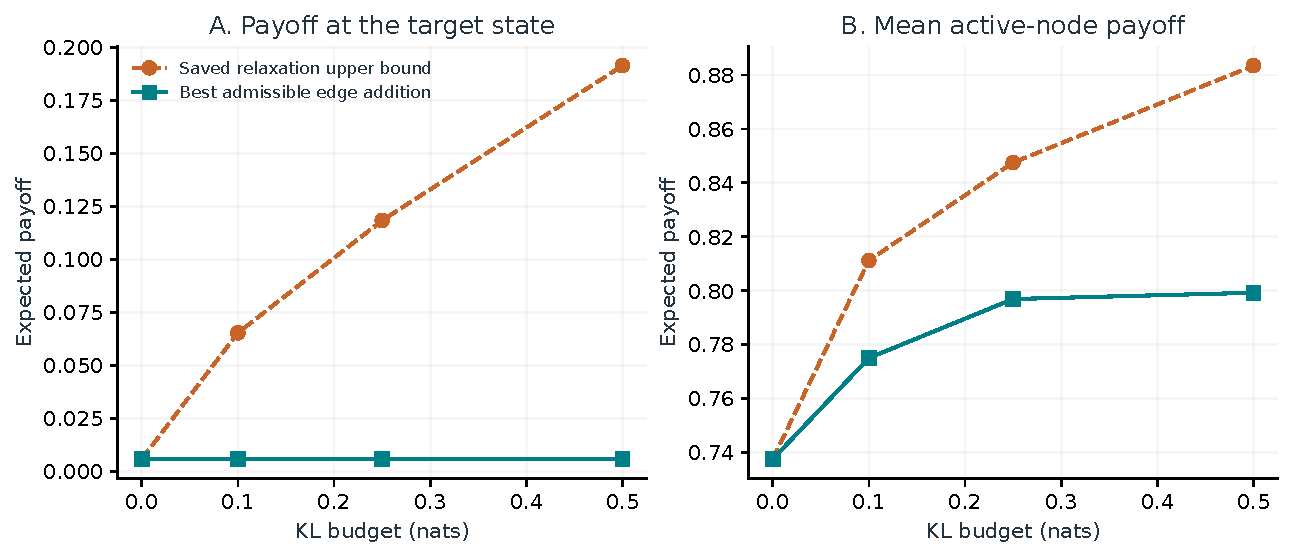
\includegraphics[width=.9\linewidth]{frontier.pdf}
\caption{Best admissible payoff and saved unrestricted upper bound for the
same catalogue. Markers are the four evaluated budgets; connecting lines
guide the eye. Panel A rewards state 0; Panel B rewards the fraction of
active nodes.}
\label{fig:frontier}
\end{figure}

The target payoff counts how often one specified message type appears.
The active-node payoff averages the proportion of features present;
it does not reward additional interactions between them.
In Figure~\ref{fig:frontier}, the catalogue curve selects the best candidate
at each budget, so it can stay flat when extra budget admits no better
choice. The stored upper bounds evaluate the ceiling in Section~2.2
over a fixed grid of $\beta$ values, with explicit boundary cases.
They need not equal the exact unrestricted optimum; displayed gaps may
include numerical slack as well as structural restriction.

\subsection{Verification and the role of complexity}
The final study covers 106,789 distinct networks, 2,400 catalogues and
105,642 changes across four families and $N=8,10,12$, with maximum
indegree five. Exact transition reconstruction, cycles, basin weights
and distributions passed the declared checks. At $C=0.25$, no nonidentity
change was feasible in 14 of 1,200 addition catalogues and 97 of 1,200
removal catalogues. Protocols and verification are in
Appendix~\ref{app:study}; complete catalogue summaries are in
Appendix~\ref{app:catalogues}.

An executable decision graph~\cite{bryant} reproduces the worked network's
10,240-bit transition table in 325 logical bits. It stores the logical
dependencies that generate the feature combinations and their transitions.
Executing it recovers every update used to calculate cycles and
distributions. Its length, called causal description length under this
encoding, measures the encoded rule structure of the complete mechanism.
This motivates the connection to Kolmogorov complexity~\cite{kolmogorov}:
an executable description gives an upper bound on the shortest programme
for the same transition table, including fixed interpreter overhead.
Equal lengths need not identify equal behaviour: feasible 339-bit
programmes yield linear payoffs from $0.737500$ to $0.796875$.
We obtain that range by grouping the feasible changes by their encoded
length and comparing their payoffs. Equal lengths can encode different
rules, so length alone cannot determine payoff in this example.
Catalogue selection uses the calculated distributions and payoffs.
The BDM comparison~\cite{bdm} and full encoding are retained in the supplement.

\section{Conclusion}
Exponential reweighting solves the stated distributional challenge, with
the alarm budget determining how far the attacker can favour higher-payoff
outcomes. The network extension evaluates the same objective over joint
feature distributions produced by permitted changes to a generator.
Cycles and basin weights determine those distributions, allowing exact
selection of the best admissible payoff within each catalogue.
The executable programme preserves the generating rules, while its length
provides a summary that need not determine payoff. The solution, constrained
experiment and description-length analysis thus have distinct, explicit roles.

\FloatBarrier
\begin{thebibliography}{9}
\bibitem{challenge} Doppel. A challenge for the 3Blue1Brown audience.
\url{https://www.3blue1brown.com/talent/doppel/}.
Accessed 12 September 2026.
\bibitem{shannon} C. E. Shannon. A mathematical theory of communication.
\emph{Bell System Technical Journal}, 27, 379--423 and 623--656, 1948.
\url{https://www.princeton.edu/~wbialek/rome/refs/shannon_48.pdf}.
\bibitem{kolmogorov} A. N. Kolmogorov. Three approaches to the quantitative
definition of information. \emph{International Journal of Computer
Mathematics}, 2, 157--168, 1968. English reprint of the 1965 paper.
\url{https://doi.org/10.1080/00207166808803030}.
\bibitem{bryant} R. E. Bryant. Symbolic Boolean manipulation with ordered
binary-decision diagrams. \emph{ACM Computing Surveys}, 24(3), 293--318,
1992. \url{https://doi.org/10.1145/136035.136043}.
\bibitem{bdm} H. Zenil, S. Hern\'andez-Orozco, N. A. Kiani,
F. Soler-Toscano and A. Rueda-Toicen. A decomposition method for global
evaluation of Shannon entropy and local estimations of algorithmic
complexity. \url{https://arxiv.org/abs/1609.00110}, version 7, 2018.
\bibitem{pybdm} PyBDM. Theory and design. Version 0.1.0 documentation.
\url{https://pybdm-docs.readthedocs.io/en/latest/theory.html}.
\end{thebibliography}
\clearpage
\appendix
\section*{Supplementary material}
\addcontentsline{toc}{section}{Supplementary material}
\label{supplement-start}
These sections provide the observation conventions, worked reconstruction,
complete experimental context and secondary analyses supporting the main
response. They introduce no additional network sample.

\section{Interpreting the distributional solution}\label{app:interpretation}
The two distributions play different roles. The fixed reference $q$
describes ordinary traffic; $p$ describes the frequencies chosen by the
attacker. Outcome $i$ denotes a phrase in the puzzle or a complete message
type in the network extension. Thus $q_i=0.3$ means that outcome $i$
accounts for 30\% of baseline messages, while $p_i=0.2$ means that the
attacker uses it in 20\% of
messages on average. Neither symbol denotes the text of a message.

The ratio $p_i/q_i$ compares the chosen frequency with the baseline.
KL divergence averages the logarithm of this ratio under $p$: it is zero
when $p=q$ and positive otherwise. The budget $C$ therefore limits how
far the attacker can shift the frequencies, as measured by this divergence.
Natural logarithms express the budget in nats.

A phrase with $q_i=0$ never occurs under the baseline model. Assigning it
positive probability would place weight on an event that the baseline
regards as impossible. The term $p_i\log(p_i/q_i)$ is then infinite, so
such a choice cannot satisfy any finite budget. We must set $p_i=0$ for
these phrases and can restrict all sums below to $q_i>0$. As usual,
terms with $p_i=0$ contribute zero to the divergence.

Here $e^{\beta s_i}$ is the exponential of $\beta s_i$: the baseline
probability $q_i$ is multiplied by this factor, not by $\beta s_i$ itself.
Larger payoffs receive larger factors, and $Z(\beta)$ makes the resulting
probabilities sum to one. For two supported phrases, their relative
frequencies satisfy
\[
 \frac{p_i(\beta)}{p_j(\beta)}
 =\frac{q_i}{q_j}\,e^{\beta(s_i-s_j)}.
\]
Thus equal payoffs preserve the baseline ratio, while a higher payoff
increases a phrase's weight relative to a lower-paying one.

Multiplication here changes a sampling weight, not the words inside a
message. Its operational interpretation is to select outcomes
with the new frequencies. For example, consider three abstract outcomes
with $q=(0.5,0.3,0.2)$ and $s=(0.1,0.4,0.9)$. At $C=0.25$,
the solution has $\beta\approx2.09644$ and
$p\approx(0.23444,0.26383,0.50173)$. In 1,000 independent selections,
the expected outcome counts change from $(500,300,200)$ to approximately
$(234,264,502)$. Individual realised counts fluctuate. The puzzle applies
its detector to the specified distribution; estimating frequencies from
a finite batch would introduce an additional sampling problem.

The parameter $\beta$ controls the strength of this preference. At
$\beta=0$ the formula gives $p=q$; increasing $\beta$ shifts probability
towards higher payoffs. It has no assigned physical meaning in this
model, whose quantities are frequencies and success probabilities.
For $\beta>0$, its mathematical role is precise: the distribution in
equation~\eqref{eq:tilt} maximises
$\E_p[s]-\KL(p\Vert q)/\beta$. Hence $1/\beta$ is the penalty placed
on divergence relative to payoff. In the interior case of Section~2.3,
choose $\beta$ so that $\KL(p(\beta)\Vert q)=C$.

\section{Network dynamics and observation model}\label{app:dynamics}
\subsection{Mapping the problem to a Boolean network}
A Boolean network contains $N$ nodes, each holding a zero or one. A local
Boolean rule determines each node's next value from its connected inputs.
All nodes update together. A network therefore defines a deterministic
function $F_A:\bits^N\rightarrow\bits^N$, where $A$ is its connectivity
matrix and the local rules are held fixed.

The adjacency matrix records these connections:
$A[\text{target}][\text{source}]=1$ when the source feeds the target
(Figure~\ref{fig:network}). We label each binary state by an integer
address $x$, running from 0 to $2^N-1$. Node $i$ has weight $2^i$, so
node 0 is the least significant bit. In the code, its value is extracted
as $(x\mathbin{\gg}i)\mathbin{\&}1$. Printed bit strings follow node order,
$x_0,\ldots,x_{N-1}$.

The ordered input repertoire lists every state once, in address order.
The corresponding output row contains the state after one update.
These ordering conventions let the decoder construct the input addresses
itself; a separate input table does not have to be transmitted.

\subsection{Why cycles define the observed frequencies}
The puzzle specifies $p$ and $q$ directly. A deterministic network instead
specifies a rule for moving between states, so we must also say how it
will be observed. Repeatedly feeding each output back as the next input
produces a trajectory. There are finitely many states, so some state must
eventually repeat. From that point onward the deterministic rule repeats
the same sequence: a \emph{cycle}. A fixed point is a cycle of length one.
The states leading to a cycle form its \emph{basin of attraction}.

To construct the distribution used in the challenge, start uniformly from
all initial states, follow the trajectory to its cycle, and choose one
position, or phase, uniformly on that cycle. If $\Gamma_A(x_0)$ is the cycle
reached from $x_0$, the resulting distribution is
\begin{equation}\label{eq:mu}
 \mu_A(x)=\frac{1}{2^N}\sum_{x_0\in\bits^N}
 \frac{\mathbf{1}\{x\in\Gamma_A(x_0)\}}{|\Gamma_A(x_0)|}.
\end{equation}
The factor $1/2^N$ gives each initial state equal weight. The indicator
selects trajectories whose eventual cycle contains $x$, and the
denominator divides that trajectory's weight among the cycle's states.
Equivalently, if a cycle has $b$ initial states in its basin and contains
$\ell$ states, each state on it has probability
\[
 \mu_A(x)=\frac{b}{2^N\ell}.
\]
Transient states have zero mass in this long-run distribution, even
though they may occur during the initial part of a trajectory.

In the challenge analogy, a network is a finite-state generator and its
state labels stand for complete message types. A cycle represents a repeated
sequence of types after the generator settles. A larger basin makes
that sequence more likely under the chosen initialisation; a longer
cycle divides its mass among more types. This is an interpretation
of the experimental generator, not a claim that natural text messages
follow Boolean cycles. Uniform initialisation and uniform phase selection
are explicit modelling choices. Figure~\ref{fig:cycles} shows how they
produce the distribution in the ten-node example.

Equation~\eqref{eq:mu} also gives the time-averaged limiting distribution
under uniform initialisation. It can differ from the distribution at one
particular late update, because different runs may have synchronised
phases. Counting output rows after just one update gives another
distribution again. We use the long-run experiment consistently for
both the baseline and each changed network.
The detector uses these marginal frequencies. It does not test the order
in which cycle states occur; a detector sensitive to temporal patterns
would pose a different problem.

Under the feature interpretation in the main text, $\mu_A$ is joint
across the nodes and marginal with respect to time: it describes a whole
feature configuration at one sampled phase, rather than a sequence of
configurations. For example, the frequency of one feature alone is found
by adding $\mu_A(x)$ over all states with that bit equal to one. Such
individual feature frequencies do not in general determine $\mu_A$.
The detector here compares the complete state distributions. A detector
using only individual feature frequencies would be a different observation
model, even though both can be constructed from the same network.

\subsection{What a perturbation changes}
A \emph{perturbation} is a specified change to the generator. Here it
means adding or removing one permitted connection while keeping the gate
types and parameters fixed. It changes which inputs a rule reads and can
therefore change the transition table, the cycles and their basin sizes.
The word \emph{disturbance} is a general informal description; we use
\emph{perturbation} for these controlled edge changes.

The baseline network $A_0$ generates $q=\mu_{A_0}$. Each permitted network
$A$ generates a candidate $p=\mu_A$. The reference $q$ stays fixed while
we compare these candidates. An edge change is an abstract modification
of the message generator's internal dependencies. It does not represent
a literal word replacement, and a single structural change need not
produce a small change in message frequencies.

Perturbations let us ask which distributions the restricted generator
can actually produce. The attacker chooses one of these changes; the
detector then compares its resulting frequencies with the original
baseline. This extends the unrestricted puzzle, in which the attacker
may choose any feasible probability vector.

\begin{table}[htbp]\centering\small
\begin{tabularx}{\linewidth}{lX}
\toprule
Challenge component & Network counterpart\\\midrule
Phrase $t_i$ & A labelled state in the common alphabet $\bits^N$\\
Ordinary distribution $q$ & $\mu_{A_0}$ for the baseline network\\
Chosen distribution $p$ & $\mu_A$ for an admissibly perturbed network\\
Phrase payoff $s_i$ & A declared state payoff $s(x)$\\
Attacker's choice & One admissible edge addition or removal\\
Judge or detector & The same rule: alarm if $\KL(\mu_A\Vert\mu_{A_0})>C$\\
Expected payoff & $\sum_x\mu_A(x)s(x)$\\
\bottomrule
\end{tabularx}
\caption{What does each part of the challenge become? The distributions,
payoff and alarm retain their mathematical roles. The attacker's available
choices acquire a structural restriction.}
\label{tab:mapping}
\end{table}

This construction preserves the distributions, payoff and alarm rule
of equation~\eqref{eq:challenge}, while restricting the available choices
to a finite set. The state labels and payoffs are declared experimental
quantities; they have not been fitted to human responses to text.
The detector applies the supplied rule to exact distributions.

For a catalogue $\mathcal{A}$ of admissible nonidentity changes, define
\begin{equation}\label{eq:frontier}
 V_{\mathcal{A}}(C)=\max_{A\in\mathcal{A}:\,
       \KL(\mu_A\Vert\mu_{A_0})\leq C}\E_{\mu_A}[s].
\end{equation}
If no change is feasible, the value is reported as unavailable. The
baseline is retained for audit but excluded from this changed-network
optimum. If taking no action is allowed, it can instead be included as an
explicit additional choice. In either convention, the unrestricted solution
provides the upper bound
\begin{equation}\label{eq:upper}
 V_{\mathcal{A}}(C)\leq U(C),\qquad
 U(C)=\inf_{\beta>0}\frac{C+\log Z(\beta)}{\beta},
\end{equation}
with the boundary cases given above. This relation is the precise link
between the original puzzle and the network experiment.

\subsection{Description length as a secondary measurement}\label{sec:length-question}
The network experiment also asks whether a short numerical description of
the generator summarises the effects of changing it. Let $R_A$ be its
complete ordered transition table and $L_A$ the logical bit length of an
executable programme that reconstructs every entry. We call $L_A$
\emph{causal description length}, with \emph{causal} referring to the known
update mechanism. This is a length under a declared encoding, not the
shortest possible programme. Its connection to Kolmogorov complexity,
including the fixed decoder overhead, is given in
Appendix~\ref{app:complexity-details}.

The distinction between the programme and its length matters. Executing
the programme recovers the transitions needed to calculate cycles,
frequencies and payoffs. Its length records how much space the encoded
rules occupy, but does not identify those rules. We therefore examine
whether equal lengths can accompany different payoffs and whether changes
in length vary with changes in the long-run distribution.

BDM provides a comparison based on patterns in the output table without
receiving the generating rules. Neither measurement enters the KL
constraint or the payoff calculation. Their role here is to assess the
limits of these summaries of the generator. Estimator conventions and
the distinction between a complete mechanism and one output are retained
in Appendix~\ref{app:complexity-details}.

\section{Network implementation and study design}\label{app:study}
\subsection{An executable representation of the generator}
The known Boolean rules are compiled into a shared ordered decision graph.
Each decision tests one input coordinate and follows a zero or one branch;
terminals supply output bits. Identical continuations are shared, following
reduced ordered binary decision diagrams~\cite{bryant}. An ordered reference
for each output makes the graph an executable description of the complete
transition table.

The index-deconvolution framework also expresses the input positions that
produce a one as decimal anchors plus additive offsets called
\emph{Sumandos}. These sets provide a way to inspect the graph and locate
output patterns. The worked example below illustrates the representation;
Appendix~\ref{app:encoding} gives the full unfolding, executable listings
and bit count. Production compilation works directly from the known
rules and need not enumerate the exported position sets.

\subsection{A worked network with ten nodes}
We use the existing baseline \texttt{ring\_n10\_s1000}, chosen by its fixed
identifier for exposition. Figure~\ref{fig:network} shows its connectivity
and dynamics. The family name denotes the study generator; this example
contains additional connections beyond a simple cycle. All gate parameter
dictionaries are empty. MAJORITY is a strict majority, so its two-input use
at node 3 requires both inputs to be one.

\paragraph{From output rows to cycles and frequencies.}
The same network has 1,024 input rows. Figure~\ref{fig:cycles} selects
rows that show how an output becomes the next input. These rows retain
their original addresses; their display order follows the cycle so that
the iteration is easy to read. For example, input 65 produces state 674,
which also appears as the output of input 321. State 65 is transient,
whereas 321 and 674 belong to the same eight-state cycle.

\begin{figure}[htbp]\centering
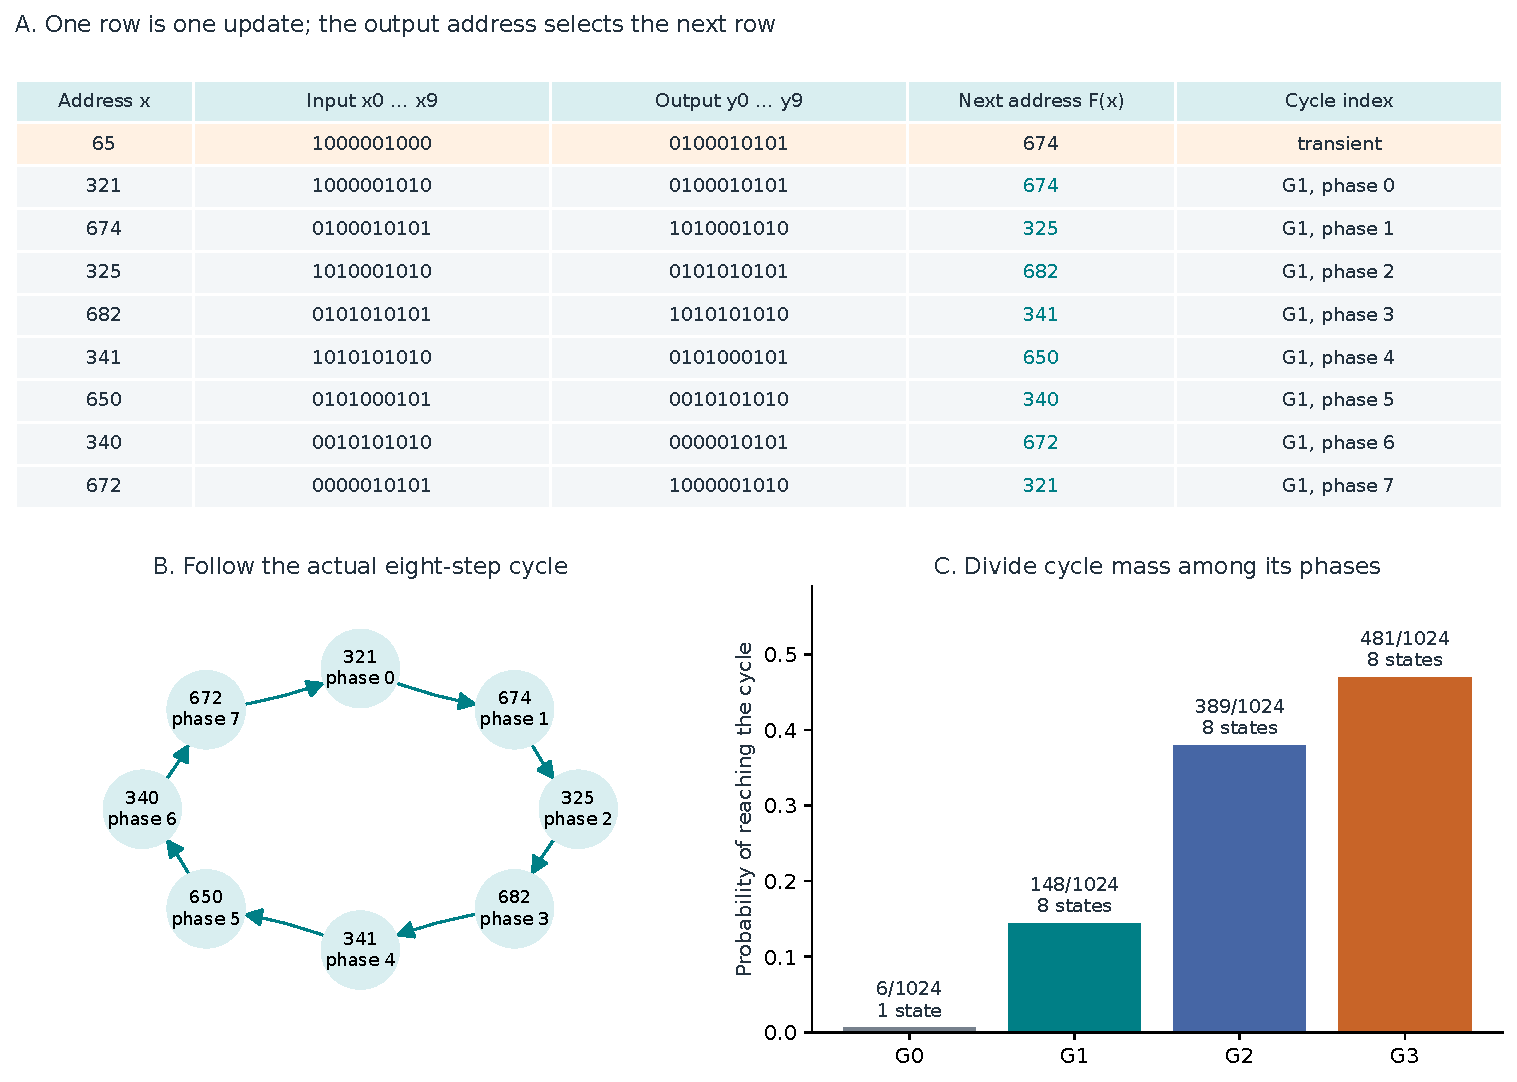
\includegraphics[width=\linewidth]{cycles_repertoire.pdf}
\caption{How does the repertoire produce a distribution? Panel A shows
selected rows, each with its input address and next-state address.
The extra cycle index records position in the trajectory, not position
in the exhaustive table. Panel B follows the actual updates through
cycle G1; phases 0--7 are labels and do not affect its probability.
Panel C gives the probability of reaching each cycle from a uniformly
chosen initial state. Dividing this mass by the number of cycle states
gives each state's long-run frequency.}
\label{fig:cycles}
\end{figure}

\begin{table}[htbp]\centering\small
\begin{tabular}{lrrrr}
\toprule
Cycle & States & Basin size & Cycle probability & Each state \\
\midrule
G0 & 1 & 6 & 3/512 & 3/512 \\
G1 & 8 & 148 & 37/256 & 37/2048 \\
G2 & 8 & 389 & 389/1024 & 389/8192 \\
G3 & 8 & 481 & 481/1024 & 481/8192 \\
\bottomrule
\end{tabular}

\caption{How much probability does each cycle receive? Basin size counts
all initial states that eventually reach that cycle, including its own
states. The four basin sizes sum to 1,024. The final column is the
probability of each individual state on the cycle, not of the cycle as
a whole.}
\label{tab:cycles}
\end{table}

Cycle G1 has a basin of 148 states and eight phases. It therefore receives
mass $148/1024$, and each phase has probability
$148/(1024\cdot8)=37/2048$. The fixed point 0 receives $6/1024=3/512$.
Together the fixed point and three eight-state cycles give 25 states with
positive long-run probability. There are 432 distinct one-step outputs,
so counting those outputs once would give a different observation model.

\paragraph{A compact description of the same transitions.}
For node 0, the output is one when an odd number of input coordinates
5, 7 and 9 are one. One branch fixes coordinates 5 and 7 to zero and
coordinate 9 to one. Its decimal anchor is 512. The other seven coordinates
are free; their additive offsets are the Sumandos, so this branch describes
128 input addresses without listing each one. Four such branches recover
all 512 addresses at which this output is one. Appendix~\ref{app:encoding}
shows the complete sets and a two-output pattern query.

Figure~\ref{fig:graph} shows the graph for output 0. It resembles a binary
tree, but branches merge when they have the same remaining computation.
The complete network has 19 reachable decision nodes, two shared terminals
and ten ordered output references. Appendix~\ref{app:programme} gives every
decision record, so the example is not dependent on a schematic drawing.

\begin{figure}[htbp]\centering
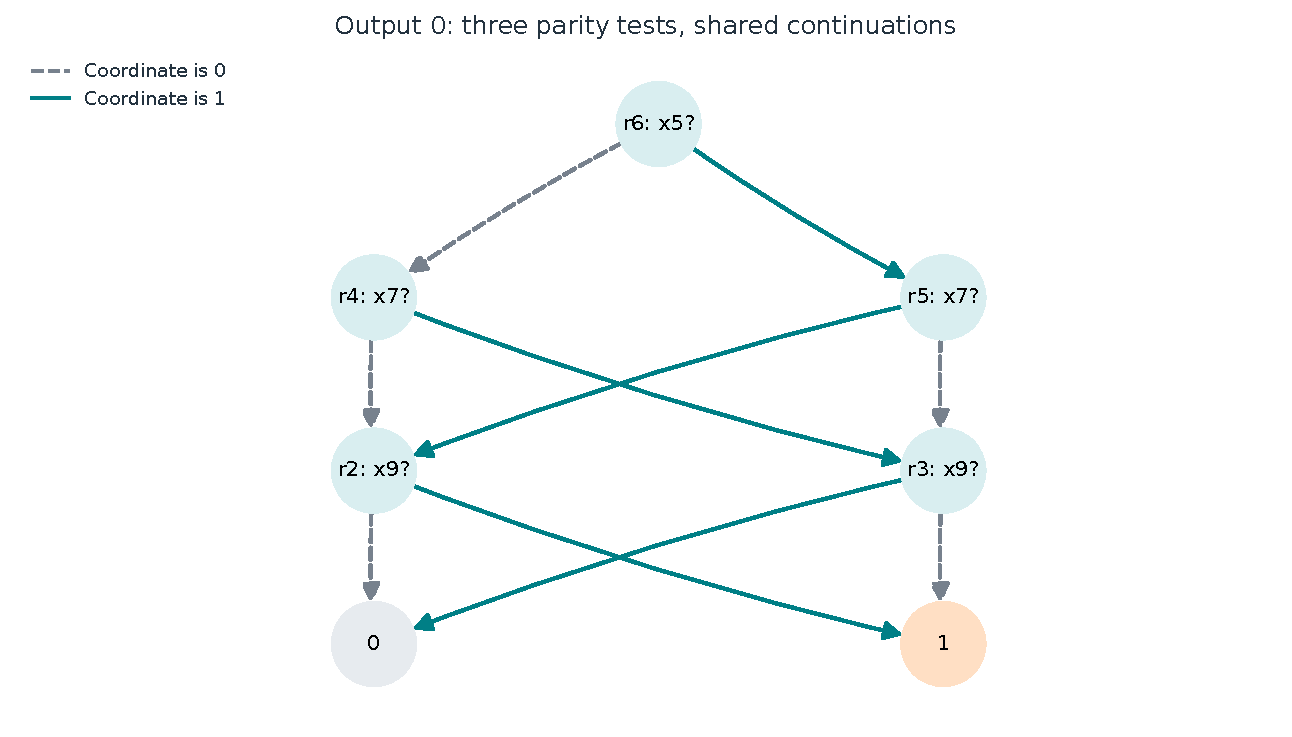
\includegraphics[width=.85\linewidth]{decision_graph.pdf}
\caption{How can several paths share a short rule? Start at reference 6 and
test the stated input coordinate. Follow the dashed branch for zero and the
solid branch for one, until reaching a terminal. A terminal is the output
bit, not a whole network state. Reused continuations keep this three-input
parity rule to five decisions. The other output references belong to the
same network programme.}
\label{fig:graph}
\end{figure}

The full graph has 19 decision nodes and uses 325 logical bits to reproduce
the 10,240-bit transition table. This demonstrates compact reconstruction
for the example. It does not establish an advantage over a direct encoding
of the connections and gates, or a speed-up in computing the long-run
distribution. For fixed $N$, the declared length formula depends only on
the number of decision nodes: equal lengths can encode different rules.
We examine the consequences of this loss of detail in the results.

\subsection{Experimental design and verification}
The first degree-five study used 240 base draws: four families, three sizes
and 20 seeds. It produced 21,380 distinct main networks and 480 catalogues.
The final replication kept the rules fixed and used 100 new seeds per
family and size, giving 1,200 base draws. Sizes were $N=8,10,12$; families
were ring, hub, modular and sparse random. The ring and hub generators keep
a structural template and vary gate assignments with seed. Consequently,
100 seeds do not mean 100 independently sampled graph structures.

Maximum indegree was five. Self-loops and empty input rows were excluded.
When a generated node exceeded that limit, a fixed selection rule retained
five input sources. The original matrix and the resulting changes were
recorded.
For every base, all one-edge additions and removals were enumerated in
separate catalogues. Gates and parameters remained fixed during perturbation;
the number of inputs and the validity of each gate were rechecked.
Unchanged baseline entries remained in the audit and were excluded from
perturbation effects and optima. When the same complete network occurred
more than once, it was evaluated once while retaining every catalogue
membership.

The main gate assignments follow the frozen family generators. All twelve
supported gates were additionally checked in a separate stress group:
AND, OR, XOR, NAND, NOR, XNOR, NOT, IMPLIES, NIMPLIES, MAJORITY, KOFN and
CANALISING. Pilot and stress results do not enter the main effect estimates.
The replication main seeds were 1000--1099 and pilot seeds were 2000--2002.

Two payoffs were used. The target payoff is one at a deterministically
chosen state with positive baseline probability and zero elsewhere.
Its expectation is the frequency of that single target message type.
The linear payoff is the fraction of active nodes in the state; its
expectation rewards states with more ones. These are two explicit
preferences over the same state alphabet, not measured probabilities
of persuading a person. KL budgets were 0, 0.1, 0.25 and
0.5 nats, with 0.25 declared primary. Infinite KL values remained explicit.
For each catalogue, the programme, BDM and dynamical changes were compared
with its own baseline.

Each unique network received a serialised programme, full network data and
an exact long-run distribution. Verification checked every output bit,
serialisation round trips, an independent trajectory calculation, cycles,
basins and rational probability mass. An independent Wolfram evaluation
checked the ordered output digest. A digest is a reproducibility identifier;
the reconstruction comparisons provide the underlying correctness evidence.

The replication initially stopped after a transaction of 48 Wolfram checks
timed out. An explicit recovery amendment retained those failed records and
repeated the 48 checks individually. Every replacement completed normally
and matched its expected digest. The final audit replayed all 110,033 pilot
and main networks with zero failures and checked 19,200 catalogue frontiers.
It rechecked the historical Wolfram evidence; it did not rerun all Wolfram
checks during this final replay. The release also passed 738 software tests
and execution of the analysis notebook.

Programme and BDM changes are measured relative to each baseline and
averaged within each base before comparing family, size and perturbation
groups. These are descriptive associations, not a test of individual
attack prediction. The estimator conventions, resampling procedure and
comparison with the earlier study are given in
Appendix~\ref{app:complexity-results}.

The explanatory extensions use the same saved ten-node baseline and its
74 edge additions. Cycle membership and basin sizes are independently
checked by following all 1,024 initial states. Row BDM is a separate
one-dimensional measurement described in Section~\ref{sec:row-complexity};
it is not mixed with the replication's matrix BDM results. The added
complexity/payoff plots recompute both payoffs and forward KL from the
saved exact probabilities. They introduce no new network sample.

\section{Additional catalogue and complexity results}\label{app:catalogues}
\subsection{Catalogue coverage and exact reconstruction}
All 106,789 main networks completed the declared reconstruction and
dynamical checks. They cover 2,400 complete nonempty catalogues and
105,642 changes relative to their baselines. Every programme reproduced
its full transition table and was shorter than the raw table in this
sample. Detailed length summaries are in
Appendix~\ref{app:complexity-results}; the payoff results below use the
exact distributions obtained from the transitions.

\subsection{The answer under a structural constraint}
For each completed catalogue, we selected the feasible change with greatest
payoff. At the primary budget, some catalogues contained no feasible
nonidentity change (Table~\ref{tab:feasible}). Keeping these cases visible
is essential to describing the attacker's actual choices.

\begin{table}[htbp]\centering\small
\begin{tabular}{llrrr}
\toprule
Change & Payoff & Catalogues & Feasible & No feasible change \\
\midrule
Add & Linear & 1200 & 1186 & 14 \\
Add & Target & 1200 & 1186 & 14 \\
Remove & Linear & 1200 & 1103 & 97 \\
Remove & Target & 1200 & 1103 & 97 \\
\bottomrule
\end{tabular}

\caption{Is there any allowed change below the alarm budget? Counts use
$C=0.25$ and all 1,200 bases per perturbation kind. Feasibility depends on
the distributional constraint, so the two payoff definitions give the same
feasibility counts. An unavailable optimum is not assigned payoff zero.}
\label{tab:feasible}
\end{table}

The ten-node example makes the distinction from the unrestricted answer
concrete. It has 74 admissible nonidentity edge additions. At $C=0.25$,
13 are feasible. For linear payoff, the selected change adds source 4 to
target 8. Its expected payoff is exactly $51/64=0.796875$, with forward
KL about 0.184507 nats. The saved unrestricted upper bound is 0.847502.
For the target payoff in this same catalogue, the best attainable value
remains 0.005859375 at each of the four budgets.

\begin{table}[htbp]\centering
\begin{tabular}{rrrr}
\toprule
KL budget & Feasible changes & Best payoff & Saved upper bound \\
\midrule
0.0 & 2 & 0.737500 & 0.737500 \\
0.1 & 12 & 0.775000 & 0.811180 \\
0.25 & 13 & 0.796875 & 0.847502 \\
0.5 & 22 & 0.799219 & 0.883444 \\
\bottomrule
\end{tabular}

\caption{What does the judge permit in the worked example? Each row uses
the same ten-node baseline and all admissible edge additions. The best
linear payoff is chosen after checking every candidate. The upper bound
describes a distributional relaxation and may be unattainable by these
edge changes.}
\label{tab:workedfrontier}
\end{table}

The stored implementation evaluates a fixed logarithmic grid in the dual
parameter, with explicit zero-budget and saturation cases. A grid value is
a conservative upper bound, not a certified exact evaluation of the
infimum in equation~\eqref{eq:upper}. The displayed gap can therefore
include numerical slack as well as a structural restriction. All 19,200
recorded frontier values or unavailable cases passed the audit; each
available optimum was below its recorded bound within the declared
numerical tolerance.

\subsection{Does description length summarise the payoff?}
Figure~\ref{fig:complexityfrontier} shows the same catalogue at the level
of individual changes. Its horizontal axis is each changed network's
\emph{actual} KL divergence, whereas Figure~\ref{fig:frontier} uses the
\emph{allowed} budget and plots the best choice below it. Its colour is
causal description length. Each point therefore answers three questions:
how far do the frequencies move, what payoff results, and how long is
the programme that generates the changed behaviour?

\begin{figure}[htbp]\centering
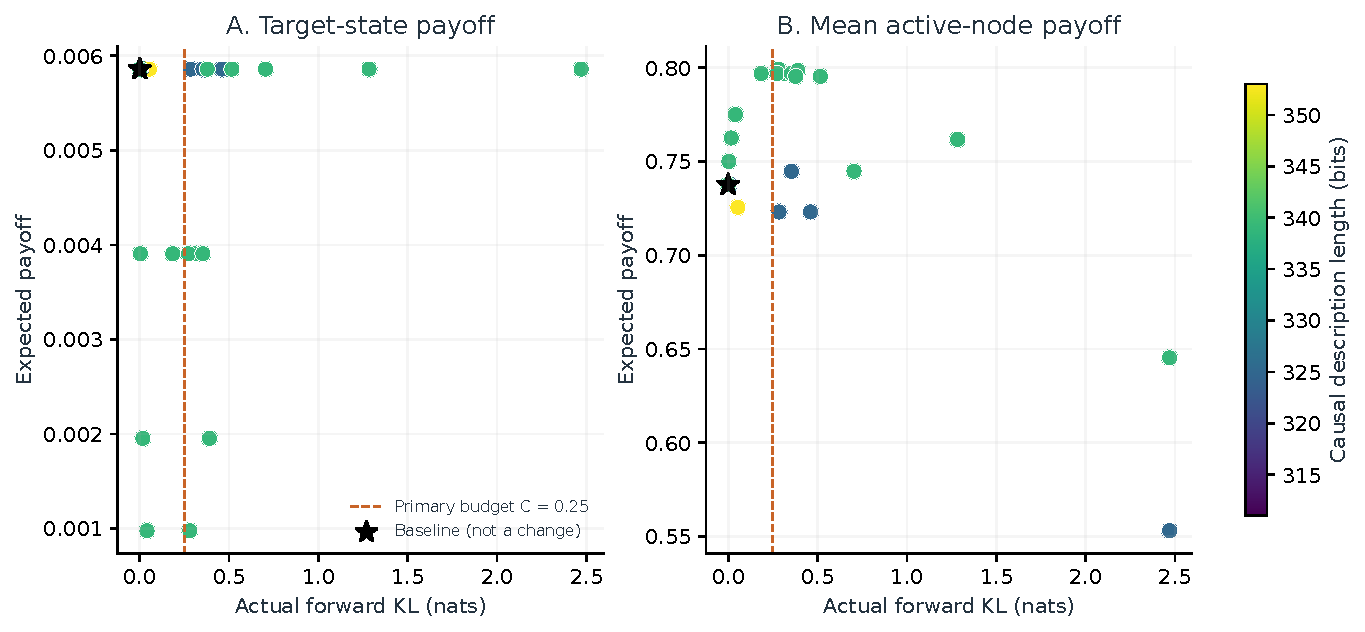
\includegraphics[width=\linewidth]{complexity_frontier.pdf}
\caption{Do generators with similar description lengths have similar
payoffs? Each coloured point is one admissible edge addition with finite
forward KL; overlapping points may hide distinct changes. Of 74 changes,
29 have finite KL and 45 introduce positive long-run mass outside the
baseline support, giving infinite KL. Those 45 cannot be placed on the
finite axis and are retained in the accompanying data. The dashed line
marks $C=0.25$; 13 changes lie on its feasible side. The black star is the
baseline for reference and is excluded from the changed-network optimum.}
\label{fig:complexityfrontier}
\end{figure}

At $C=0.25$, feasible programme lengths are 325, 339 and 353 bits.
Among 339-bit programmes, linear payoff ranges from 0.737500 to 0.796875.
The 353-bit feasible programme gives 0.725521. Thus length alone does not
rank the payoff: different rules can require the same number of encoded
bits yet produce different distributions. The selected source-4-to-target-8
addition uses 339 bits and achieves the best linear payoff at this budget.
It has target-state payoff $1/256$, so improving the linear objective
does not also optimise the target objective.

These examples show that description length alone is insufficient to
determine payoff in this catalogue. The graph retains the specific rules
that produce the distribution; the bit count discards that detail.
Length measures a stored representation, not attack effort or persuasive
power. There is no programme length assigned to the unrestricted bound,
because its distribution need not be generated by a network in the
catalogue. Appendix~\ref{app:3d} retains the three-dimensional view of
the same observations.

\subsection{What the replication adds}
Across every family/size group, mean programme length and mean matrix BDM
increased under edge addition and decreased under removal. Their detailed
responses were not interchangeable: correlations between base-mean
programme and BDM changes ranged from $-0.011$ to $0.618$, while those
between programme changes and total variation ranged from $-0.432$ to
$0.327$. Appendix~\ref{app:complexity-results} gives the full comparisons.

These results describe associations between averages within each base.
Total variation measures distributional change; the detector instead uses
forward KL. The correlations therefore neither establish independence
nor test whether complexity predicts detection of an individual change.
Together with the worked example, they limit a universal interpretation
of length as a summary of behaviour. They do not show that adding
complexity improves the choice of an attack.

\section{Programme encoding and worked reconstruction}\label{app:encoding}
\subsection{From index rules to an executable description}
The method represents where output bits are one, then uses those
positions to reconstruct each row. The index-deconvolution framework
describes sets of row positions through
decimal anchors and additive offsets called \emph{Sumandos}. A compact
schema fixes some bit coordinates and leaves others free. If $a$ stores
the fixed one-bits and $m$ stores the free coordinates, then
\begin{equation}\label{eq:schema}
 S(m)=\left\{\sum_{i:m_i=1}\epsilon_i2^i:\epsilon_i\in\bits\right\},
 \qquad P(a,m)=\{a+s:s\in S(m)\},\qquad a\mathbin{\&}m=0.
\end{equation}
The decimal anchor records the fixed one-bits. The mask identifies the
coordinates that are free to vary, and generates the additive offsets;
it is not itself a list of Sumandos. Adding these offsets to an anchor
unfolds the schema into input addresses. A union of schemas specifies
the one positions of an output column; the remaining positions are zero.
Reading all columns at the same address recovers the complete output
row, including which node values occur together.

In this study the rules are known. The compiler turns them directly into
an ordered decision graph, using node coordinates in
ascending order. Each decision has a coordinate, a zero child and a one
child. Identical branches are removed and identical continuations are
shared, following reduced ordered binary decision diagrams~\cite{bryant}.
Ten outputs use ten ordered references into the same graph. There is one
programme for the network.

For teaching, the graph can be exported as decimal/free-mask schemas and
rebuilt from them. Production compilation need not enumerate those schemas,
their Sumandos, input assignments or possible output patterns. This distinction
matters: a parity function may have many accepting paths but a short graph.
The graph and the schemas describe the same input--output map. We measure
the length of the executable graph encoding, including the information
needed to decode it, rather than counting displayed anchors alone.

\paragraph{From a short rule to its addresses.}
For node 0, the output is one precisely when an odd number of coordinates
5, 7 and 9 are one. Its anchors are $[512,128,32,672]$. Every anchor has
free mask $351=1+2+4+8+16+64+256$, generating
\begin{equation}
 S(351)=\{0,\ldots,31\}\cup\{64,\ldots,95\}
       \cup\{256,\ldots,287\}\cup\{320,\ldots,351\}.
\end{equation}
Thus the decimal/Sumandos representation for this column is
\[
[\text{decimals},\text{Sumandos}]=[[512,128,32,672],S(351)].
\]
Each anchor contributes 128 positions. The four sets are disjoint and
contain 512 positions in total. For instance, anchor 512 fixes coordinates
5 and 7 to zero and coordinate 9 to one. Adding each offset fills in the
seven free coordinates.

\begin{figure}[htbp]\centering
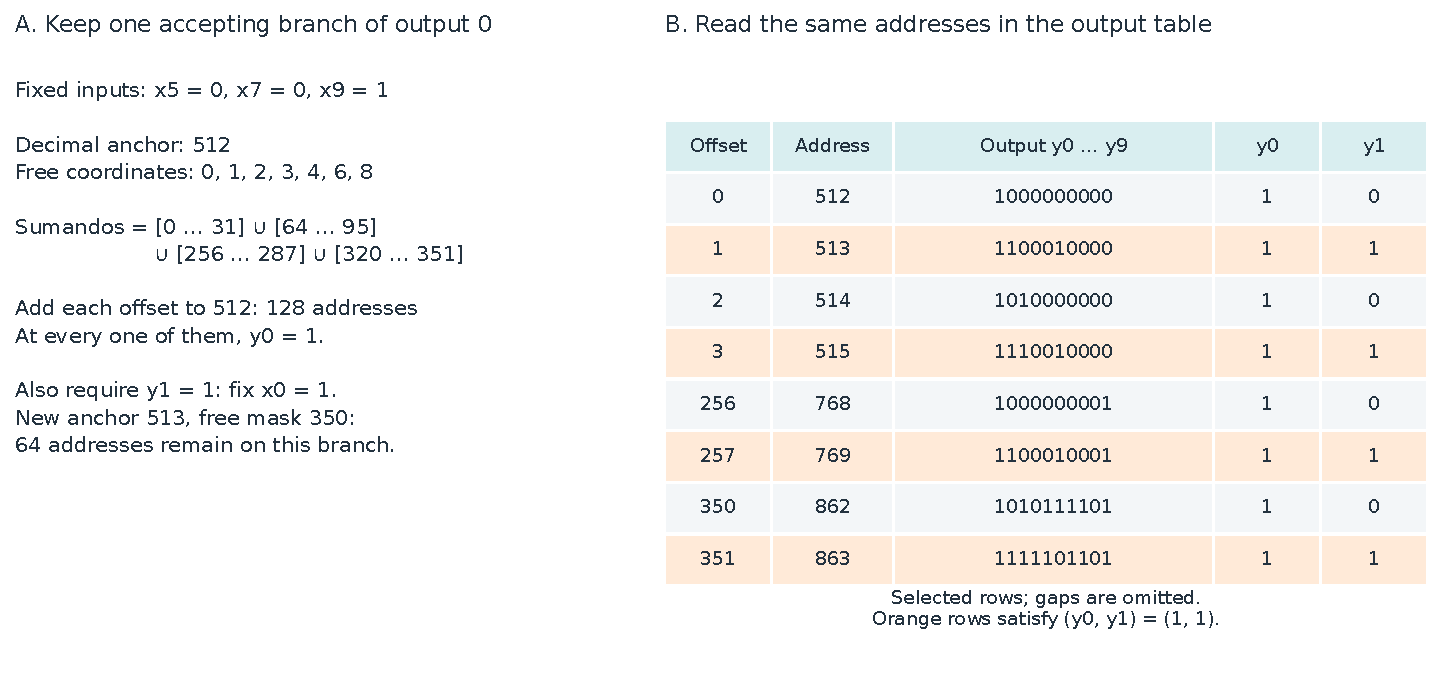
\includegraphics[width=\linewidth]{schema_unfolding.pdf}
\caption{How do decimals and Sumandos locate an output pattern? One
accepting XOR branch fixes three input coordinates. Its anchor 512 plus
128 offsets identifies rows with $y_0=1$. Requiring $y_1=1$ also fixes
$x_0=1$, leaving 64 rows on that branch. The displayed rows are selected
examples, not the complete unfolded set; their output bits come from
the verified network.}
\label{fig:unfolding}
\end{figure}

This also supports a simple subpattern query. Node 1 copies input 0, so
requiring $(y_0,y_1)=(1,1)$ restricts the XOR one positions to addresses
with $x_0=1$. On the branch above, the anchor becomes 513 and the free
mask becomes 350. Across all four XOR branches, the full query is
\[
 \bigcup_{a\in\{513,129,33,673\}}\{a+s:s\in S(350)\},
\]
containing exactly 256 input addresses. The purpose is to locate which
inputs generate a pattern. It does not change the network or introduce
a new distribution by itself.
\begin{table}[htbp]\centering\small
\begin{tabular}{rlp{8cm}r}
\toprule
Output & Gate & Decimal anchors and free masks & One positions \\
\midrule
0 & XOR & (512, 351), (128, 351), (32, 351), (672, 351) & 512 \\
1 & AND & (1, 1022) & 512 \\
2 & XOR & (2, 1021) & 512 \\
3 & MAJORITY & (5, 1018) & 256 \\
4 & AND & (8, 1015) & 512 \\
5 & XOR & (16, 1006), (1, 1006) & 512 \\
6 & OR & (32, 983), (8, 1015) & 768 \\
7 & XOR & (64, 959) & 512 \\
8 & OR & (128, 895) & 512 \\
9 & OR & (256, 703), (64, 959) & 768 \\
\bottomrule
\end{tabular}

\caption{Which positions are one in each output? Each pair is
(decimal anchor, free-coordinate mask), rather than two explicit offset
lists. Generate all submasks of the mask and add them to the anchor.
The union within a row specifies one output column. All ten rows together
specify the complete output table.}
\label{tab:schemas}
\end{table}

\FloatBarrier
The following executable operations show both routes. The source network is
saved with the manuscript evidence. The final assertion checks every one of
the 10,240 output bits against the direct gate implementation.

\begin{minipage}{\linewidth}
\begin{lstlisting}
from doppel_challenge.adapters import Network, repertoire
from doppel_challenge.repertoire_program import (
    compile_repertoire_program, compile_schema_program,
    export_output_schemata, serialize_program,
    deserialize_program, iter_output_rows)

# spec contains the saved connectivity, gates and parameters.
net = Network(n=10, C=spec['cm'], gates=spec['dyn'],
              params=spec['params'])
programme = compile_repertoire_program(net)
schemas = [export_output_schemata(programme, j)
           for j in range(10)]
payload = serialize_program(programme)
assert serialize_program(compile_schema_program(10, schemas)) == payload
restored = deserialize_program(payload, n=10)
rows = list(iter_output_rows(restored))
assert rows == repertoire(net)
print("Rows:", len(rows), "Output bits:", len(rows) * 10)
print("Output 0 schemas:", schemas[0])
\end{lstlisting}

\begin{lstlisting}[language={}]
Rows: 1024 Output bits: 10240
Output 0 schemas: [(512, 351), (128, 351), (32, 351), (672, 351)]
\end{lstlisting}
\end{minipage}

For an explicit unfolding of one schema, use:

\begin{minipage}{\linewidth}
\begin{lstlisting}
anchor, mask = 512, 351
offsets, s = [], mask
while True:
    offsets.append(s)
    if s == 0:
        break
    s = (s - 1) & mask
positions = sorted(anchor + s for s in offsets)
assert len(positions) == 128
assert all(rows[x][0] == 1 for x in positions)
subpattern = [x for x in positions if rows[x][1] == 1]
assert len(subpattern) == 64
print("Sumandos:", sorted(offsets)[:4], "...",
      sorted(offsets)[-4:])
print("Positions:", positions[:4], "...", positions[-4:])
print("Branch rows with (y0,y1)=(1,1):", len(subpattern))
print("At input 513:", rows[513])
\end{lstlisting}

\begin{lstlisting}[language={}]
Sumandos: [0, 1, 2, 3] ... [348, 349, 350, 351]
Positions: [512, 513, 514, 515] ... [860, 861, 862, 863]
Branch rows with (y0,y1)=(1,1): 64
At input 513: [1, 1, 0, 0, 0, 1, 0, 0, 0, 0]
\end{lstlisting}
\end{minipage}

Repeating this construction for all ten columns recovers every transition.
The resulting programme is a compressed representation of the original
behaviour, not a newly inferred wiring diagram. Iterating those transitions
then determines the cycles and the distribution used by the detector.
This is the connection between the decimal/Sumandos representation,
causal description length and the challenge.

\subsection{Measuring the binary programme}
We count the information needed to store and run the representation.
For $M$ decision nodes, the codec stores a self-delimiting count,
$M$ coordinate-and-child records, and $N$ output references. Let
$v=\lceil\log_2 N\rceil$ and $r=\lceil\log_2(M+2)\rceil$. Its logical
length is
\begin{equation}\label{eq:length}
 L_A=2\lfloor\log_2(M+1)\rfloor+1+M(v+2r)+Nr.
\end{equation}
The count uses an Elias-gamma code for $M+1$, which tells the decoder
where that field ends without a separate length marker. Coordinate and reference
fields use fixed-width, least-significant-bit-first representations.
Decision identifiers follow a fixed order: children before their parent,
zero before one, and outputs in column order. This removes arbitrary
numbering differences, so equal reachable graphs under these conventions
give equal serialisations.

For the example, $M=19$, $v=4$, $r=5$. Table~\ref{tab:bits} shows every
contribution. The programme occupies 41 bytes after adding three padding
bits. The raw table is already binary: $10\times1024=10,240$ bits. The
logical programme uses about 3.17\% of that length. No input table, network
topology, gate labels or parameters are supplied to the decoder.

\begin{table}[htbp]\centering
\begin{tabular}{lr}
\toprule
Field & Logical bits \\
\midrule
Node-count code & 9 \\
Decision records & 266 \\
Ordered output references & 50 \\
Total programme & 325 \\
Raw ordered output & 10240 \\
Byte padding (separate) & 3 \\
\bottomrule
\end{tabular}

\caption{What exactly is counted? The 325 logical bits contain enough
structure to interpret the decisions and recover all ten outputs.
The three padding bits only fill the last byte. The fixed interpreter
overhead in equation~\eqref{eq:kolmogorov} remains unmeasured.}
\label{tab:bits}
\end{table}

Counting only bare anchors and offsets would measure a different object
unless their grouping and output association were also supplied. The
executable codec makes that decoding structure explicit. Compression is
not guaranteed for every object: the same codec has a three-node
AND/OR/XOR benchmark of 54 programme bits against 24 raw bits. A valid
description may be longer than its data. No raw-table fallback is used.

\subsection{What computation is saved?}
Producing a compact rule and listing everything it generates are different
computational tasks. The compiler can produce the exact description without writing the
$N2^N$-bit table. For the supported local gates, parity uses a number of
construction states proportional to indegree $d$, and threshold rules use
at most order $d^2$ states. Reading the current dense adjacency input
already costs order $N^2$. These observations explain why a compact
representation is practical, while distinguishing that task from reading
every output.

A query for one output row traverses the decisions needed by each output;
in this direct local-gate setting it uses at most order $Nd$ decisions.
Printing the full table requires at least $N2^N$ bit writes. General Boolean
composition, schema export and long-run inference do not inherit a universal
linear-time guarantee. The present compiler also supports a specified gate
library rather than arbitrary function minimisation. We make no numerical
speed-up claim against another complete implementation in this paper.

Compilation is symbolic, but the experimental correctness checks, dynamics
and BDM materialise the complete small-network output tables. The distinction
allows exact validation without treating the cost of validation as the cost
of producing the compact description.

\section{Interpretation of the complexity measurements}\label{app:complexity-details}
\subsection{Why measure causal description length?}
Shannon's information theory relates probabilities to average coding
cost~\cite{shannon}. KL divergence measures the expected log probability
ratio between two distributions. Here it supplies the constraint on changing
frequencies. Its units are nats because the logarithm is natural.

Algorithmic information theory asks how short a programme can be while
still generating a particular object~\cite{kolmogorov}. Let $R_A$ be the
ordered matrix with row $x$ equal to $F_A(x)$. We measure the logical binary
length $L_A$ of a programme that reconstructs $R_A$. Define
$\CDL(A):=L_A$ under the stated compiler, codec and ordering conventions.
This is the \emph{causal description length} used here. We use \emph{causal
complexity} only with this operational meaning, not as a new expression
for the exact Kolmogorov complexity. For a fixed universal
interpreter $U$, this yields
\begin{equation}\label{eq:kolmogorov}
 K_U(R_A\mid N,\text{ordering})\leq L_A+c_U,
\end{equation}
where $c_U$ includes the fixed decoder and interpreter overhead. Our codec
is self-delimiting given $N$. The bound follows by supplying the valid
programme to that decoder. The experiment measures $L_A$; it does not
measure $c_U$ or find the shortest programme among all possible programmes.

Its value is to quantify how much explicit rule structure is needed by
our representation to reproduce every transition. We can test that
description by executing it. Comparing $L_A$ with the raw table length
measures compression; comparing $L_A-L_{A_0}$ across perturbations shows
how this description changes when the mechanism changes.

The full transition table determines the trajectories and thus
equation~\eqref{eq:mu}. The reverse need not hold. Different transition
tables can have the same long-run distribution. Complexity of $R_A$ and
divergence of $\mu_A$ therefore describe different properties. A change in
programme length alone does not determine whether the judge raises an alarm.

\subsection{Why compare with BDM?}
The Block Decomposition Method estimates algorithmic complexity by dividing
an object into small blocks, assigning each distinct block a precomputed
coding-theorem estimate, and accounting for repetition~\cite{bdm,pybdm}.
In schematic form it uses $\sum_b[\operatorname{CTM}(b)+\log_2 n_b]$,
where $n_b$ counts copies of block $b$. Our programme instead gives an
explicit exact description built from the known Boolean rules. Comparing
their responses to the same perturbations tests whether these two
descriptions of regularity vary together. BDM is an estimate in its own
units; it is not the stored length of our programme.

The comparison is useful because the two methods obtain their descriptions
differently. Our method uses the known generating rules and provides an
executable reconstruction. BDM examines patterns in the output object
without receiving those rules. Agreement under perturbation suggests
that some changes in the explicit description are also visible to the
block estimator. Disagreement may reflect their different representations,
block sizes or sensitivity to shared structure. Neither outcome measures
accuracy against the unknown shortest programme.

Complexity is not needed to derive the solution in Section~2.1, and the
specified detector never consults it. In the network experiment it is an
additional description of the generator: how much rule structure
accompanies a given payoff and distributional change? Treating complexity
as an extra detection signal or an attacker cost would require a new
model and a separate evaluation.

\subsection{One output is not the whole mechanism}\label{sec:row-complexity}
There are three different objects that an output-complexity measurement
might refer to: one $N$-bit row $y=F_A(x)$, one node's column across all
$2^N$ inputs, or the complete $2^N\times N$ transition table $R_A$.
The measurements must name which object they describe.

Write $P_A$ for the network programme. It generates every row when given its input address.
For a fixed interpreter and ordering, this gives
\[
 K_U(F_A(x)\mid x,N,\text{ordering})\leq L_A+c_{\mathrm{eval}}.
\]
The same upper bound works for every $x$. It does not say that the shortest
programme for each row has that length. For example, a row of ten zeros
can be generated without reproducing the rest of the network. More
generally, storing the ten output bits literally provides another
description, with its own fixed decoding overhead.

If $x$ is not supplied, a programme using the network must also specify
which input to evaluate. Consequently,
\[
 K_U(F_A(x)\mid N,\text{ordering})
 \leq L_A+K_U(x\mid N,\text{ordering})+O(1).
\]
If the network programme itself is supplied as auxiliary information,
evaluating one row given $x$ requires only a fixed evaluator:
$K_U(F_A(x)\mid x,P_A,N,\text{ordering})=O(1)$.
These are different questions because different information is supplied.

Assigning $L_A$ to every row is therefore meaningful as a label for the
shared generating mechanism, not as a separate estimate of each row's
intrinsic complexity. Once that mechanism is transmitted, it can be reused
for all inputs. Dividing its cost by the number of queries would describe
an amortised communication cost, not the Kolmogorov complexity of a row.
Similarly, an executable description of one output column could retain
only the rules needed by that node. It need not cost as much as the
whole network, and separately encoding all columns can duplicate shared
rules.

BDM applied to each row instead asks about regularity within each short
output string. Whole-table BDM also sees blocks spanning several rows
and columns; summing row scores does not reproduce that measurement.
For an illustrative check on the ten-node example, we additionally
measure each output row with one-dimensional BDM using a single ten-bit
block, without padding. At this size the score is the lookup estimate
for that block~\cite{pybdm}; it is distinct from the two-dimensional
$4\times4$ convention used in the main experiment.

\begin{table}[htbp]\centering\small
\begin{tabular}{rrlrr}
\toprule
Input $x$ & Output $F_A(x)$ & Output bits & Row BDM & $L_A$ (bits) \\
\midrule
0 & 0 & \texttt{0000000000} & 22.784 & 325 \\
65 & 674 & \texttt{0100010101} & 25.988 & 325 \\
321 & 674 & \texttt{0100010101} & 25.988 & 325 \\
512 & 1 & \texttt{1000000000} & 23.933 & 325 \\
513 & 35 & \texttt{1100010000} & 26.676 & 325 \\
1023 & 991 & \texttt{1111101111} & 24.578 & 325 \\
\bottomrule
\end{tabular}

\caption{What remains fixed when output strings differ? Selected input
addresses identify rows in the same ten-node network. Row BDM evaluates
the displayed ten-bit string. The last column repeats the 325-bit
network programme length as a mechanism label; it is not a measured
minimum description length of that row. Inputs 65 and 321 give the same
output and therefore the same row score.}
\label{tab:rowcomplexity}
\end{table}

Across all 1,024 rows, there are 432 distinct outputs and row BDM ranges
from 22.784 to 29.428. The constant mechanism label and varying row scores
show that one fixed generator can produce strings with different local
regularities. These very short-string estimates do not establish
differences in message meaning, persuasiveness or detection risk. Under
a different assignment of binary labels to message types, their
values could change even when the outcome probabilities and payoffs are
preserved.

\section{Supplementary complexity results}\label{app:complexity-results}
\subsection{Estimator and comparison conventions}
BDM used \texttt{pybdm} version 0.1.0 on the original output matrix, with
non-overlapping $4\times4$ blocks and \texttt{PartitionIgnore} after zero
padding. For $N=10$, the $1024\times10$ matrix was padded to
$1024\times12$, adding 2,048 zero bits; $N=8$ and $N=12$ needed no padding.
Padding is recorded as a BDM convention and is excluded from raw and
programme lengths. For the worked example, BDM is 675.95 in BDM units.

Effects were averaged within each base and perturbation kind, then equally
across bases in each family/size/kind group. The 95\% intervals use 5,000
seeded resamples of base draws and describe sampling stability. They are
not perturbation-level significance tests. The previous and final studies
are compared group by group, without pooling them. Network-wide length
summaries below are descriptive summaries of distinct stored networks.

\subsection{The exact programme retains the full output table}
All 106,789 main networks completed the declared checks. There were 2,400
complete nonempty catalogues of permitted changes and 105,642 changes
relative to their baselines. The programme
was shorter than raw for every main network in this sample.
Table~\ref{tab:lengths} reports the full range of programme lengths, including
the longest cases. These are exact lengths under the codec conventions.

\begin{table}[htbp]\centering\small
\begin{tabular}{rrrrr}
\toprule
$N$ & Networks & Raw bits & Programme bits: min / median / max & BDM median \\
\midrule
8 & 21,204 & 2,048 & 65 / 257 / 439 & 609.94 \\
10 & 34,832 & 10,240 & 131 / 339 / 695 & 733.52 \\
12 & 50,753 & 49,152 & 199 / 419 / 787 & 1053.74 \\
\bottomrule
\end{tabular}

\caption{How large are the complete output and its programme? Each row
summarises distinct main networks of one size. The BDM median describes the
original output matrix under the declared block and padding convention. It
does not measure bits transmitted by the programme.}
\label{tab:lengths}
\end{table}

\begin{figure}[htbp]\centering
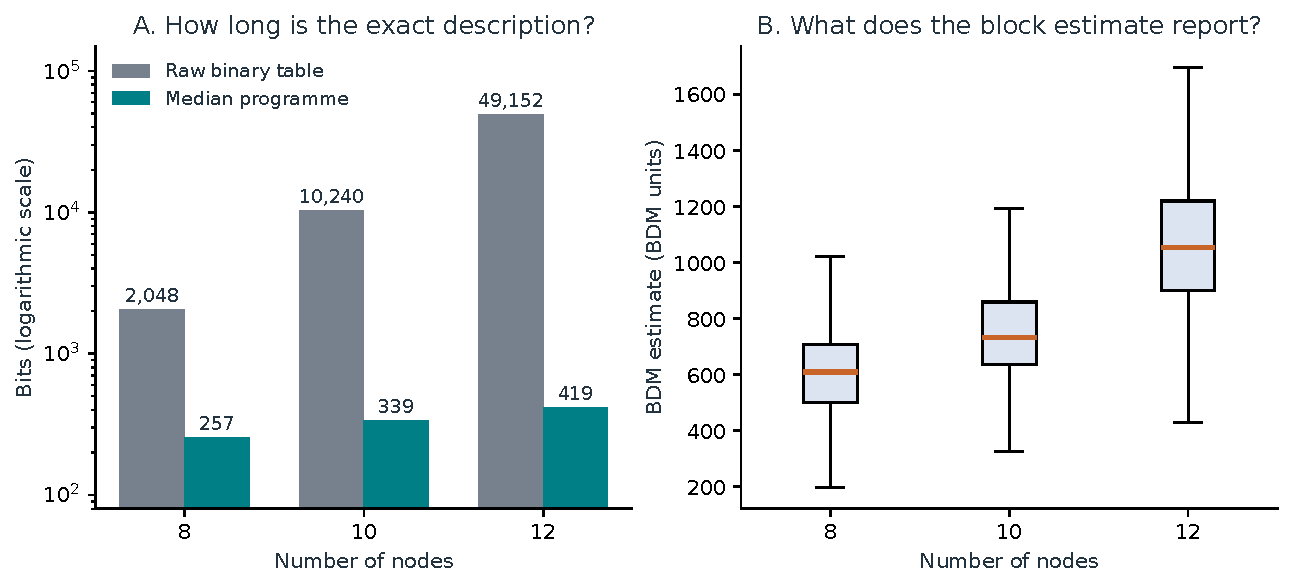
\includegraphics[width=\linewidth]{lengths_bdm.pdf}
\caption{How much smaller is the exact generative description? Panel A
compares raw length with median programme length on a logarithmic bit axis;
labels give the actual values. Panel B shows BDM on its own axis: the box
contains the middle 50\%, the line is the median, and whiskers extend to
the most extreme observations within 1.5 interquartile ranges. Outlier
points are omitted from the drawing, not from the data or calculations.}
\label{fig:lengths}
\end{figure}

The ratios fall with $N$ over this design because the exhaustive table
grows exponentially while each local rule remains bounded in indegree.
This result supports compact reconstruction for these networks. It does
not establish compactness for arbitrary output tables or remove the cost
of exhaustive long-run analysis.

\subsection{Programme length, BDM and behaviour under perturbation}
Mean causal description length and mean matrix BDM increased under addition and decreased
under removal in every family/size group of the final replication. These
are group means, not a statement that every single edge change has the
same sign. Figure~\ref{fig:effects} places these effects alongside the
change in the long-run distribution.

\begin{figure}[htbp]\centering
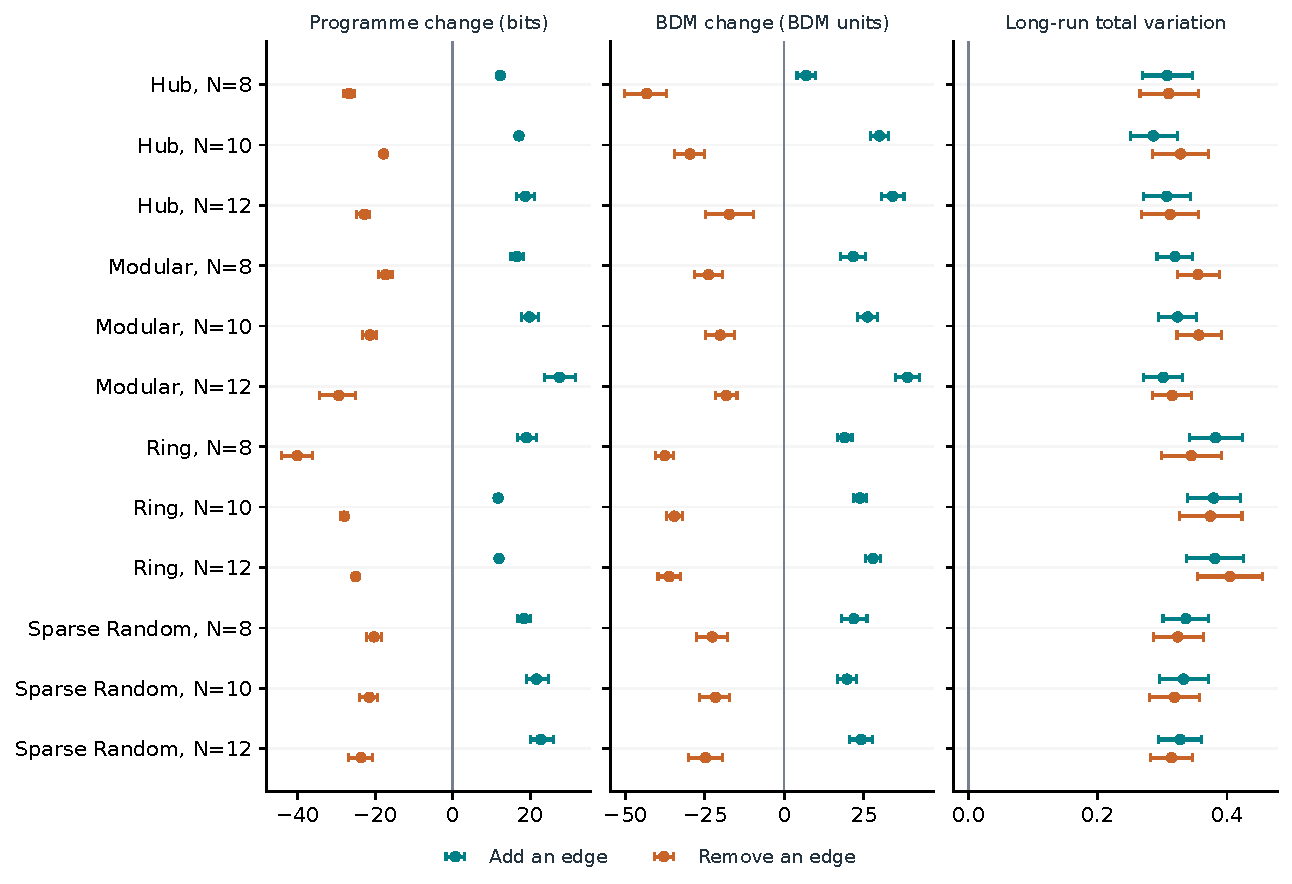
\includegraphics[width=\linewidth]{effects.pdf}
\caption{Do longer descriptions accompany larger behavioural changes?
Read across each family and size. Teal points describe addition; orange
points describe removal. Each point is an equally weighted mean of 100
base means, and each interval uses the declared base resampling procedure.
The panels measure different quantities. In particular, total variation
measures distributional change and has no sign corresponding to whether
programme length increases or decreases.}
\label{fig:effects}
\end{figure}

Agreement in average signs does not make the measures interchangeable.
Across the 24 groups, Spearman correlations of base-mean programme changes
with base-mean BDM changes range from $-0.011$ to $0.618$. Correlations
between programme changes and total variation range from $-0.432$ to
$0.327$. Thus the relation depends on family, size and perturbation kind.
These descriptive associations do not establish a detection advantage or
an accuracy ranking against an unknown Kolmogorov complexity.

\subsection{Comparison with the earlier study}
The final study increases base draws fivefold while retaining the same
design. Table~\ref{tab:replication} reports the range of changes in the 24
matched group means. Complete group values are retained in the released
comparison table; these ranges are descriptive differences and carry no
cross-group significance claim. Appendix~\ref{app:groups} gives all final
group means.

\begin{table}[htbp]\centering\small
\begin{tabular}{lrr}
\toprule
Quantity & Smallest change & Largest change \\
\midrule
Programme/raw (percentage points) & -0.182 & 1.043 \\
Programme effect (bits) & -4.696 & 6.180 \\
BDM effect (BDM units) & -8.154 & 11.260 \\
Total variation effect & -0.019 & 0.082 \\
\bottomrule
\end{tabular}

\caption{How much did the estimates change in the larger replication?
Values are final minus previous group means. The smallest and largest
differences may come from different groups. No perturbation rows are
treated as independent replication units.}
\label{tab:replication}
\end{table}

\FloatBarrier
\section{The complete worked programme}\label{app:programme}
References 0 and 1 are terminals. Each row below is a decision record.
The output references for nodes 0 through 9 are
\[
 [6,7,8,10,11,14,16,17,18,20].
\]
Together with $N=10$ and the stated ordering, these records define the
complete output table. The canonical programme digest is
\begin{center}\footnotesize\ttfamily
2271d1949e4e957370e8faddf94fed16d87b1cef5d0aaff60810f3aba22589b2
\end{center}
\begin{center}\small\input{generated/decisions.tex}\end{center}

\section{All final group means}\label{app:groups}
Programme/raw is the mean ratio after averaging perturbations within each
base. $\Delta L$ is measured in bits; $\Delta$BDM uses BDM units; TV is total
variation of the long-run distributions. Additions and removals are separate.
There are 100 base draws in each row.
\begin{center}\small\begin{tabular}{lrlrrrr}
\toprule
Family & $N$ & Change & $L/|R|$ (\%) & $\Delta L$ & $\Delta$BDM & TV \\
\midrule
hub & 8 & Add & 14.38 & 12.28 & 6.91 & 0.308 \\
hub & 8 & Remove & 12.48 & -26.68 & -43.27 & 0.310 \\
hub & 10 & Add & 3.71 & 17.09 & 29.93 & 0.286 \\
hub & 10 & Remove & 3.37 & -17.80 & -29.70 & 0.328 \\
hub & 12 & Add & 0.93 & 18.70 & 34.07 & 0.307 \\
hub & 12 & Remove & 0.85 & -22.80 & -17.28 & 0.312 \\
modular & 8 & Add & 9.43 & 16.53 & 21.71 & 0.319 \\
modular & 8 & Remove & 7.78 & -17.35 & -23.85 & 0.355 \\
modular & 10 & Add & 3.34 & 19.81 & 26.18 & 0.323 \\
modular & 10 & Remove & 2.94 & -21.34 & -20.15 & 0.356 \\
modular & 12 & Add & 1.06 & 27.54 & 38.75 & 0.301 \\
modular & 12 & Remove & 0.95 & -29.44 & -18.21 & 0.315 \\
ring & 8 & Add & 11.80 & 19.02 & 18.99 & 0.382 \\
ring & 8 & Remove & 8.91 & -40.12 & -37.53 & 0.345 \\
ring & 10 & Add & 3.14 & 11.74 & 23.78 & 0.379 \\
ring & 10 & Remove & 2.75 & -28.00 & -34.59 & 0.374 \\
ring & 12 & Add & 0.77 & 11.94 & 27.90 & 0.381 \\
ring & 12 & Remove & 0.69 & -25.08 & -36.10 & 0.404 \\
sparse random & 8 & Add & 13.37 & 18.40 & 21.89 & 0.336 \\
sparse random & 8 & Remove & 11.48 & -20.30 & -22.66 & 0.324 \\
sparse random & 10 & Add & 3.79 & 21.61 & 19.69 & 0.333 \\
sparse random & 10 & Remove & 3.37 & -21.57 & -21.63 & 0.319 \\
sparse random & 12 & Add & 0.92 & 22.75 & 24.18 & 0.328 \\
sparse random & 12 & Remove & 0.82 & -23.65 & -24.77 & 0.314 \\
\bottomrule
\end{tabular}
\end{center}

\section{A three-dimensional view of the worked catalogue}\label{app:3d}
\begin{figure}[htbp]\centering
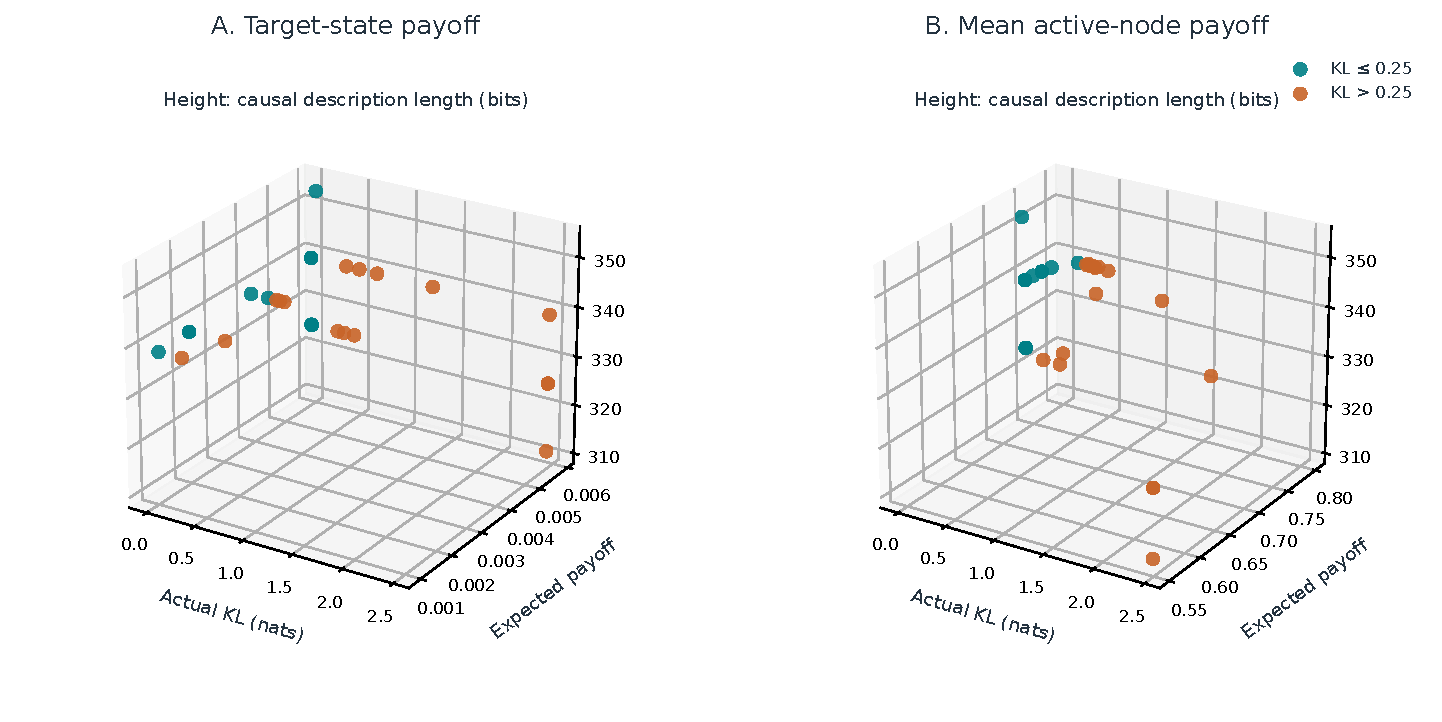
\includegraphics[width=\linewidth]{complexity_frontier_3d.pdf}
\caption{What does complexity add as a third coordinate? Height gives
causal description length for the same 29 finite-KL changes shown in
Figure~\ref{fig:complexityfrontier}. Teal points satisfy the primary
budget; orange points exceed it. The 45 infinite-KL cases remain outside
this finite plot. Each point is a complete changed network, not an
individual message or output row. No surface is fitted between points.}
\label{fig:3d}
\end{figure}

Points at the same height share an encoded length, not necessarily a
programme or a distribution. Points with the same payoff can also have
different lengths. The third coordinate therefore describes the mechanism
associated with a candidate choice; it does not change the detector's
feasibility rule. A preference for shorter programmes among equally
successful choices would be an additional optimisation criterion.




% \FloatBarrier
% \section{Data and reproducibility}
% The primary results are stored in
% \path{doppel-challenge/results/joint_degree5_final_replication_analysis_v1}.
% The comparison study is
% \path{doppel-challenge/results/joint_degree5_final_analysis_v1}.
% Their release records seal the analysis, tests, executed notebooks and
% underlying evidence. The earlier N=6 study is historical and is excluded
% from the denominators of this manuscript.

% The manuscript script verifies both releases and compares their declared source
% hashes before generating its evidence. Historical notebook evidence comes from
% the archived, hash-verified executed snapshots. Later differences in editable
% copies are recorded in the manuscript evidence file. The script
% rechecks all 10,240 bits of the
% worked example, reconstructs the same programme from its exported schemas,
% checks their positions for exactness and duplicates within each output,
% and recomputes the selected worked payoff and KL from saved rational
% probabilities. Generated tables, figure PDFs, full worked outputs and
% checksums are supplied alongside the source.

% The additional explanatory module reconstructs the cycle order from the
% transition map, checks all basin sizes independently and verifies the
% two-output subpattern by exhaustive comparison. It records all 1,024
% row BDM values and recomputes the 74 worked-catalogue payoffs and
% divergences from exact probabilities. These checks and the separate
% row-estimator convention are saved in the manuscript evidence. The
% printed code outputs are checked against actual execution.

% From the repository root, run:
% \begin{lstlisting}[language={}]
% PYTHONPATH=doppel-challenge/src python \
%   doppel-challenge/paper/response_v1/build_evidence.py
% latexmk -pdf -interaction=nonstopmode -halt-on-error -cd \
%   doppel-challenge/paper/response_v1/main.tex
% PYTHONPATH=doppel-challenge/src python doppel-challenge/paper/response_v1/verify_draft.py
% \end{lstlisting}
% The first command derives manuscript evidence from completed experiments.
% It does not launch another network study. The frozen protocols, seeds,
% admissibility rules and recovery amendment are part of the accompanying
% repository evidence.


\end{document}
